\section{Forschungsdesign}
\begin{figure}[htb!]
    \begin{center}
        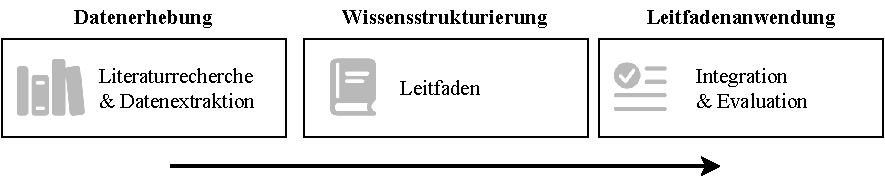
\includegraphics[width=\textwidth]{contents/03_research_design/res/research_design_overview.pdf}
    \end{center}
    \caption{Überblick des Forschungsdesigns}
    \label{fig:research_design_overview}
\end{figure}

Eine Übersicht der Vorgehensweise zur Beantwortung der Forschungsfragen ist in \autoref{fig:research_design_overview} dargestellt. Der Forschungsansatz besteht aus zwei wesentlichen zusammenhängenden Teilen.

Zunächst wurden Daten zum aktuellen Wissensstand über die Aspekte von Erklärungen sowie dessen Zusammenhänge und Auswirkungen auf Softwarequalität erhoben. Zu diesem Zweck wurde eine Literaturrecherche mittels der Suchstring-Methode \cite{kitchenham2004procedures} durchgeführt. Die Antworten auf die Forschungsfragen sind aus den selektierten Arbeiten extrahiert worden, wobei zunächst die Forschungsfragen RQ1-RQ3 bearbeitet wurden, um darauf aufbauend die Fragen nach den Einflüssen (RQ4.1 und RQ4.2) zu beantworten.

Auf Basis der Resultate dieser Datenerhebung konnten die Ergebnisse zu den ersten drei Forschungsfragen in ein Modell über die Aspekte von Erklärbarkeit überführt werden. Dies orientiert sich sowohl an Strukturen, welche die Literaturrecherche ergeben hat, als auch an den Forschungsfragen und der Definition von Erklärbarkeit von \citeauthor{chazette_knowledge_nodate} \cite{chazette_knowledge_nodate} (siehe \autoref{sec:model_explanation_aspects}).

Die erhobenen Daten zur Beantwortung der Forschungsfragen RQ4.1 und RQ4.2 sind in einem Katalog der Zusammenhänge zwischen Rahmenbedingen, Charakteristiken von Erklärungen und dem Einfluss auf ausgewählt externe  Qualitätsaspekte gebündelt. Als Schlussfolgerung daraus wurden außerdem Design-Empfehlungen abgeleitet.

\bigbreak

Der zweite Teil der Forschung besteht aus der Anwendung des entstandenen Leitfadens zur Prüfung, ob dieser die Integration von Erklärungen in ein bestehendes System unterstützt. Ziel war es, dass neu integrierte Erklärungen sich positiv auf zuvor mithilfe des Leitfadens definierte Qualitätsziele auswirken.

Die Prüfung der Praxistauglichkeit des Leitfadens wurde zusammen mit dem Unternehmen \textit{Graphmasters GmbH} \footnote{\url{https://www.graphmasters.net}, besucht: 10.09.21} aus Hannover durchgeführt. \textit{Graphmasters} ist unter anderem das entwickelnde Unternehmen hinter der Navigationssoftware \textit{NUNAV Navigation} \footnote{\url{https://www.nunav.net}, besucht: 10.09.21}, welches ein Smartphone-Navigationssystem für Endnutzer mit einem kollaborativen Routing-Ansatz ist (Für mehr Details siehe \autoref{sec:model_evaluation}).

Zunächst wurden bestehende Nutzungsprobleme von \textit{NUNAV} analysiert. Darauf basierend hat ein interdisziplinäres Team von \textit{Graphmasters} in einem vorbereiteten Workshop (siehe \nameref{ch:appendix_1}) anhand des zuvor entwickelten Leitfadens grundlegende Ideen für Erklärungen gesammelt. Mithilfe dieser konnten konkrete Anforderungen abgeleitet werden.

Auf Basis der Ergebnisse wurden dann mehrere Erklärungstypen entwickelt und in NUNAV integriert. Diese sind im nächsten Schritt in einer \textit{Case Study} mit Nutzern des Systems evaluiert worden.

Als Abschluss der Forschung wurde zur besseren Interpretation der qualitativen Ergebnisse der \textit{Case Study} ein nicht repräsentatives qualitatives Experiment (Quasi-Experiment) unter Nutzern von \textit{NUNAV Navigation} durchgeführt.

\bigskip

In den folgenden Kapiteln werden die einzelnen beschriebenen Schritte zusammen mit den Ergebnissen näher erläutert.